\documentclass[journal,12pt,twocolumn]{IEEEtran}

\usepackage{setspace}
\usepackage{gensymb}
\singlespacing
\usepackage[cmex10]{amsmath}

\usepackage{amsthm}

\usepackage{float}
\usepackage{mathrsfs}
\usepackage{txfonts}
\usepackage{stfloats}
\usepackage{bm}
\usepackage{cite}
\usepackage{cases}
\usepackage{subfig}
% \usepackage[demo]{graphicx}
% \usepackage{caption}
% \usepackage{subcaption}
\usepackage{longtable}
\usepackage{multirow}

\usepackage{enumitem}
\usepackage{mathtools}
\usepackage{steinmetz}
\usepackage{tikz}
\usepackage{circuitikz}
\usepackage{verbatim}
\usepackage{tfrupee}
\usepackage[breaklinks=true]{hyperref}
\usepackage{graphicx}
\usepackage{tkz-euclide}

\usetikzlibrary{calc,math}
\usepackage{listings}
    \usepackage{color}                                            %%
    \usepackage{array}                                            %%
    \usepackage{longtable}                                        %%
    \usepackage{calc}                                             %%
    \usepackage{multirow}                                         %%
    \usepackage{hhline}                                           %%
    \usepackage{ifthen}                                           %%
    \usepackage{lscape}     
\usepackage{multicol}
\usepackage{chngcntr}

\DeclareMathOperator*{\Res}{Res}
\renewcommand\thesection{\arabic{section}}
\renewcommand\thesubsection{\thesection.\arabic{subsection}}
\renewcommand\thesubsubsection{\thesubsection.\arabic{subsubsection}}

\renewcommand\thesectiondis{\arabic{section}}
\renewcommand\thesubsectiondis{\thesectiondis.\arabic{subsection}}
\renewcommand\thesubsubsectiondis{\thesubsectiondis.\arabic{subsubsection}}


\hyphenation{op-tical net-works semi-conduc-tor}
\def\inputGnumericTable{}                                 %%

\newtheorem{theorem}{Theorem}[section]
\newtheorem{problem}{Problem}
\newtheorem{proposition}{Proposition}[section]
\newtheorem{lemma}{Lemma}[section]
\newtheorem{corollary}[theorem]{Corollary}
\newtheorem{example}{Example}[section]
\newtheorem{definition}[problem]{Definition}

\newcommand{\BEQA}{\begin{eqnarray}}
\newcommand{\EEQA}{\end{eqnarray}}
\newcommand{\define}{\stackrel{\triangle}{=}}
\bibliographystyle{IEEEtran}
\raggedbottom
\setlength{\parindent}{0pt}
\providecommand{\mbf}{\mathbf}
\providecommand{\pr}[1]{\ensuremath{\Pr\left(#1\right)}}
\providecommand{\qfunc}[1]{\ensuremath{Q\left(#1\right)}}
\providecommand{\sbrak}[1]{\ensuremath{{}\left[#1\right]}}
\providecommand{\lsbrak}[1]{\ensuremath{{}\left[#1\right.}}
\providecommand{\rsbrak}[1]{\ensuremath{{}\left.#1\right]}}
\providecommand{\brak}[1]{\ensuremath{\left(#1\right)}}
\providecommand{\lbrak}[1]{\ensuremath{\left(#1\right.}}
\providecommand{\rbrak}[1]{\ensuremath{\left.#1\right)}}
\providecommand{\cbrak}[1]{\ensuremath{\left\{#1\right\}}}
\providecommand{\lcbrak}[1]{\ensuremath{\left\{#1\right.}}
\providecommand{\rcbrak}[1]{\ensuremath{\left.#1\right\}}}
\theoremstyle{remark}
\newtheorem{rem}{Remark}
\newcommand{\sgn}{\mathop{\mathrm{sgn}}}
% \providecommand{\abs}[1]{\left\vert#1\right\vert}
\providecommand{\res}[1]{\Res\displaylimits_{#1}} 
% \providecommand{\norm}[1]{\left\lVert#1\right\rVert}
%\providecommand{\norm}[1]{\lVert#1\rVert}
\providecommand{\mtx}[1]{\mathbf{#1}}
% \providecommand{\mean}[1]{E\left[ #1 \right]}
\providecommand{\fourier}{\overset{\mathcal{F}}{ \rightleftharpoons}}
%\providecommand{\hilbert}{\overset{\mathcal{H}}{ \rightleftharpoons}}
\providecommand{\system}{\overset{\mathcal{H}}{ \longleftrightarrow}}
	%\newcommand{\solution}[2]{\textbf{Solution:}{#1}}
\newcommand{\solution}{\noindent \textbf{Solution: }}
\newcommand{\cosec}{\,\text{cosec}\,}
\providecommand{\dec}[2]{\ensuremath{\overset{#1}{\underset{#2}{\gtrless}}}}
\newcommand{\myvec}[1]{\ensuremath{\begin{pmatrix}#1\end{pmatrix}}}
\newcommand{\mydet}[1]{\ensuremath{\begin{vmatrix}#1\end{vmatrix}}}
\numberwithin{equation}{subsection}
\makeatletter
\@addtoreset{figure}{problem}
\makeatother
\let\StandardTheFigure\thefigure
\let\vec\mathbf
\renewcommand{\thefigure}{\theproblem}
\def\putbox#1#2#3{\makebox[0in][l]{\makebox[#1][l]{}\raisebox{\baselineskip}[0in][0in]{\raisebox{#2}[0in][0in]{#3}}}}
     \def\rightbox#1{\makebox[0in][r]{#1}}
     \def\centbox#1{\makebox[0in]{#1}}
     \def\topbox#1{\raisebox{-\baselineskip}[0in][0in]{#1}}
     \def\midbox#1{\raisebox{-0.5\baselineskip}[0in][0in]{#1}}

\lstset{
%language=C,
frame=single, 
breaklines=true,
columns=fullflexible
}
\title{Assignment 6}
\author{Varenya Upadhyaya EP20BTECH11026}
\date{}
\begin{document}

\maketitle
Download all python codes from:
\begin{lstlisting}
https://github.com/varenya27/AI1103/blob/main/Assignment6/codes
\end{lstlisting}
and all latex-tikz codes from:
\begin{lstlisting}
https://github.com/varenya27/AI1103/blob/main/Assignment6/main.tex
\end{lstlisting}
\maketitle   
\begin{center}
\section{\textbf{Problem}}
\end{center}
Let $Y_1$ denote the first order statistic in a random sample of size $n$ from a distribution that has the pdf, 
\begin{align}
    f(x) = \nonumber
    \begin{cases}
    e^{-(x-\theta)}&\text{ when } \theta<x<\infty\\
    0 &\text{  otherwise} 
    \end{cases}
\end{align}
Obtain the distribution of $Z_n = n(Y_1 - \theta)$\\
\maketitle
\section{\textbf{Solution}}
The first order statistic for any sample is the the minimum of the given sample 
In order to calculate the distribution for $Y_1$, we need the the cumulative distribution function $F(x)$ of x:\\
\begin{align}
  F(x) &=\displaystyle\int\limits_{-\infty}^{x} f(t) \,dt\\
  &= \displaystyle\int\limits_{-\infty}^{\theta}0\,dt + \displaystyle\int\limits_{\theta}^{x}e^{\theta-t}\,dt\\
  &=\brak{e^{\theta-t}}_{x}^{\theta}\\
  &= 1-e^{\theta-x} \\
  &= 1-f(x)
\end{align}
This gives: 
\begin{align}
    F(x) = 
    \begin{cases}
    1-e^{-(x-\theta)} &\text{when }\theta<x<\infty\\
    0 &\text{otherwise}
    \end{cases}
\end{align}
Now,
\begin{align}
    F(x) = \pr{X\leq x}\\
    \implies 1-F(x) = \pr{X>x}
\end{align}
In the random sample of size $n$, $Y_1$ can take $n$  values. For $Y_1 = x$, all the other terms must be greater than $x$. Let $Q(x)$ be the distribution for $Y_1$:

\begin{align}
    Q(x) &= n\times f(x)\times\left[\prod_{i=1}^{n-1}\pr{X_i>x}\right]\\
    &= n f(x)\times[1-F(x)]^{n-1}\\
    &= n(f(x))^{n}
\end{align}
Thus,
\begin{align}
    Q(x) = \label{eq_1}
    \begin{cases}
    n(e^{-n(x-\theta)})&\text{when }\theta<x<\infty\\
    0 &\text{otherwise }
    \end{cases}
\end{align}
\begin{figure}[h!]
    \centering
    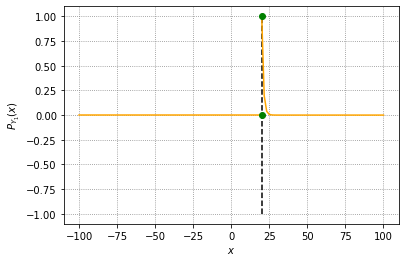
\includegraphics[width = \columnwidth]{Y1_1.png}
    \caption{Distribution when $n=1$}
    \label{fig:fig_1}
\end{figure}

\begin{figure}[h]
    \centering
    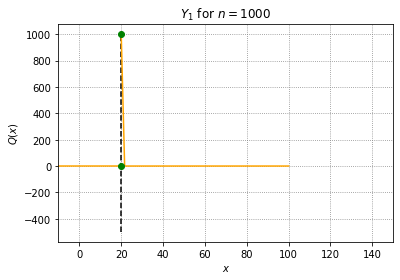
\includegraphics[width = \columnwidth]{Y1_1000.png}
    \caption{Distribution as $n$ increases to 1000}
    \label{fig:fig_2}
\end{figure}
Fig. \ref{fig:fig_1} and Fig. \ref{fig:fig_2} are the plots for the function in \eqref{eq_1} when $\theta=20$. It can be seen that as $n$ approaches infinity, the function becomes a vertical line at $x=\theta$ \\

The required distribution is $Z_n$:
\begin{align}
    Z_n &= n(Y_1 - \theta)\\
    &=\label{eq_2}
    \begin{cases}
    n(n(e^{-n(x-\theta)})-\theta)&\text{when }\theta<x<\infty\\
    0 &\text{otherwise}
    \end{cases}
\end{align}
Fig. \ref{fig:fig_3} and Fig. \ref{fig:fig_4} are the plots for the distribution in \eqref{eq_2} for $\theta=20$
\begin{figure}[h]
    \centering
    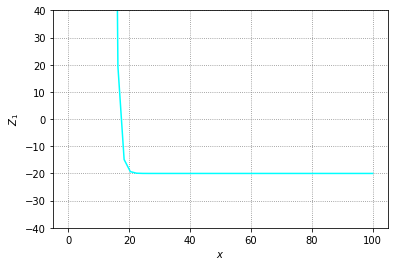
\includegraphics[width=\columnwidth]{Z_1.png}
    \caption{$Z_n$ when $n=1$}
    \label{fig:fig_3}
\end{figure}
\begin{figure}[H]
    \centering
    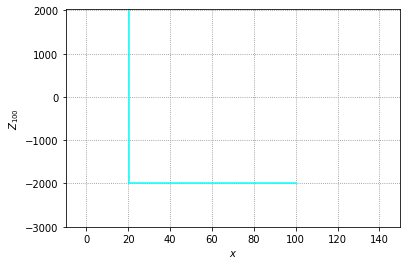
\includegraphics[width=\columnwidth]{Z_100.png}
    \caption{$Z_n$ when $n=100$}
    \label{fig:fig_4}
\end{figure}

\end{document}